\section{Prompt Design}
\label{sec:method}
We describe the iterative methodology of designing prompts with users' feedback, which will be listed in bullet point in this section. 

% Our prompt engineering for chatbots was based on (i) the objectives proposed by psychiatrists (see Section \ref{sec:objectives}), (ii) the process of ``trial and error'', and (iii) the feedback of psychiatrists. In this part, we will discuss the design process in detail.
% \KZ{I'm assuming in the trial and error stage, you will involve
% the human doctors and patients and get their feedback. But how is this process
% actually playing out? How is it different from the final evaluation which also
% consists of human and automatic evaluation. It's a little confusing.
% I think sec 4 - 7 need to be re-organized according to the two-stage
% methodology and redesign what to put into the final evaluation section.}
% In this part, we will discuss the design process in detail.


\subsection{Doctor Chatbot}

\begin{figure}[th]
	\centering
	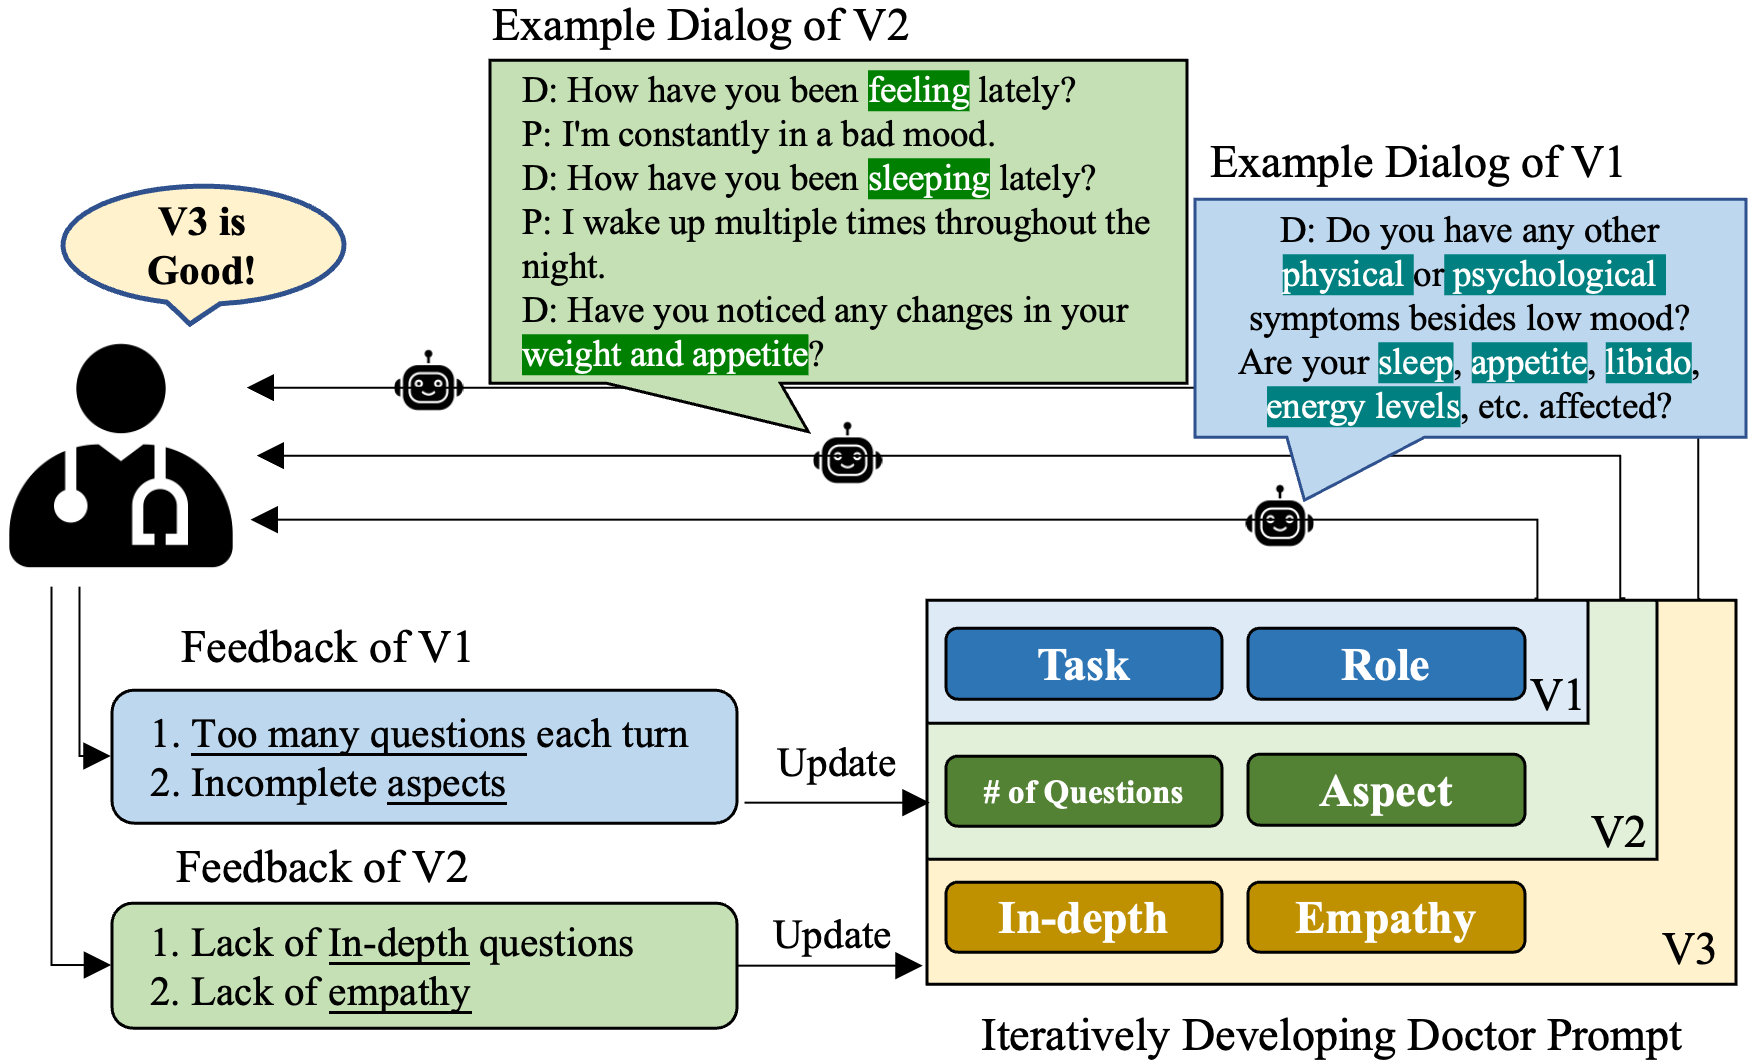
\includegraphics[width=\linewidth]{Figures/doctor_prompt_design.png}
	\caption{The iterative development process of the prompt of doctor chatbots. Psychiatrists will identify the limitations of the current version, and we will address these issues in the subsequent version.}
	\label{fig:doc_prompt_design}
\end{figure}

\label{sec:doc_prompt}
\paragraph{Version 1}
The original version of the prompt for doctor chatbot is as follows. We simply describe the task without providing any other information. 
\begin{prompt}
    \textcircled{1} Please play the \uline{role} of a psychiatrist. 
    \textcircled{2} Your \uline{task} is to conduct a professional diagnosis conversation with me based on the DSM-5 criteria. 
\end{prompt}
% However, the typical question of the doctor chatbot induced by this prompt is
% \begin{quote}
% \small
%     ``Do you have any other physical or psychological symptoms besides low mood? Are your \Pink{sleep, appetite, libido, energy levels, etc.} affected? Do you have any \Pink{family} members who have had similar issues?''
% \end{quote}
% \MY{can we put the prompt analyses into bullet points or just paragraph like :Strengths, Drawbacks for each version update? I think in this way, we can make prominent updates clearly and possibly remove some verbose expressions}
\begin{itemize}
    \item Although the chatbot's questions are in line with DSM-5\cite{american2013diagnostic}, it asks about almost all symptoms in one go (See Example V1 in Figure \ref{fig:doc_prompt_design}), which can be overwhelming for the patient. 
    \item Additionally, the chatbot draws a diagnosis conclusion in less than five turns without gathering sufficient information, which may result in unreliable diagnostic outcomes and fail to achieve the objective of ``comprehensiveness''.
\end{itemize}

\paragraph{Version 2}
Therefore, we developed a new version to address these problems by adding sentence \textcircled{3} and \textcircled{4} (i.e., ``ques num'' and ``aspect'' in Figure \ref{fig:doc_prompt_design}) to the original prompt. 
\begin{prompt}
    \textcircled{3} Your questions should \uline{cover at least the following aspects}: [\ldots]\protect\footnotemark. 
    % You are free to choose the order of questions, but you must collect complete information on all aspects in the end. 
    \textcircled{4} Please only ask \uline{one question at a time}.
    % , and each question should only cover one symptom.
\end{prompt}
\footnotetext{We will provide the full list in the Appendix.}
% \KZ{The english sounds strange in this table.}
\begin{itemize}
    \item After the modification, the doctor chatbot does satisfy the requirements in the prompt, but it appears indifferent to the patient's input and mechanically transits to the next aspect without offering empathy or support (see example V2 in Figure \ref{fig:doc_prompt_design}).
    \item Moreover, psychiatrists also emphasize the importance for the doctor chatbot to ask in-depth questions. For example, if a patient expresses feeling down, the chatbot should ask the follow-up question, ``How long have you been experiencing this mood?'' to gain a better understanding of the symptom, rather than inquiring next symptom immediately.
\end{itemize}

% \begin{table}[h]
%     \centering
%     \footnotesize
%     \begin{tabular}{m{0.18\columnwidth}|m{0.68\columnwidth}}
%     \hline
%     Doctor bot & Can you tell me the \Pink{emotional issues} you've been experiencing recently?  \\
%     \hline
%     Patient & It feels like I'm constantly in a bad mood. \\
%     \hline
%     Doctor bot & How have you been \Pink{sleeping} lately? Have you noticed any issues? \\
%     \hline
%     Patient & I've been waking up multiple times throughout the night. \\
%     \hline
%     Doctor bot & Have you noticed any changes in your \Pink{weight and appetite}?\\
%     \hline
%     \end{tabular}
%     \caption{Example dialogue fragment of doctor chatbot empowered by the Version 2 prompt.}
%     \label{tab:example_prompt}
% \end{table}

\paragraph{Version 3}
Therefore, we focus on empathy and in-depth questioning in the upcoming version.

% In OpenAI's example prompt, it defines an ``AI assistant'' with several characteristics (e.g., The assistant is helpful, creative, clever and very friendly). Inspired by this, 
We first modify sentence \textcircled{1} as ``Please play a role of an \uline{empathetic and kind} psychiatrist''. Then, we add sentences \textcircled{5}\textcircled{6} to the previous version.
\begin{prompt}
    \textcircled{5} You need to ask \uline{in-depth questions}, such as the \Blue{duration}, \Blue{causes} and specific \Blue{manifestations}. 
    \textcircled{6} You need to use various \uline{empathetic strategies}, such as \Yellow{understanding}, \Yellow{support} and \Yellow{encouragement}. % COMMENT: encouragement?
\end{prompt}
We include examples (highlighted in colored boxes) in the prompt to guide the doctor chatbot in asking in-depth questions and demonstrating empathy. These examples are crucial because, without them, the chatbot tends to ask superficial questions and  rely on a generic phrase like ``thank you very much for your answer'' to show empathy. This arises from ChatGPT's limited comprehension of ``in-depth questioning'' and ``empathy'' in clinical contexts. Consequently, providing examples can be a promising approach to help ChatGPT grasp certain specialized skills within professional domains.
% COMMENT: 这些词汇叫做example吗?感觉会和ICL中的范例exemplar混淆

% We believe that this issue arises from ChatGPT's limited understanding of ``in-depth questioning'' and ``empathy'' in clinical scenarios. The examples serve as a guide for the chatbot to inquire additional information and express empathy when needed. 
Since this version fulfills the three requirements for doctor chatbots, we deem it the final iteration\footnote{The final version is in Table \ref{tab:doctor_prompt} in the Appendix.}. 

% \KZ{I remember you mentioned that in the middle of the conversation, we may need
% to insert some additional instruction to ChatGPT to reinforce these instructions
% because it can forget? You didn't mention these here.}

\subsection{Patient Chatbot}
\label{sec:pat_prompt}

\paragraph{Version 1}
The original version of the prompt for patient chatbot is as follows. 
\begin{prompt}
    \textcircled{1} Please play the \uline{role} of a patient, who is currently chatting with a doctor. 
    \textcircled{2} \uline{You are experiencing the following symptoms}: [\texttt{Symptom List}]\protect\footnotemark 
    % \KZ{How did ChatGPT summarize these symptoms? Shall we trust the symptoms given by ChatGPT?}
    \textcircled{3} Please talk to me based on the above symptom list. 
    \textcircled{4} You can only mention \uline{one symptom per round}. 
\end{prompt}
\footnotetext{The symptom list is summarized by ChatGPT and revised by psychiatrists. See Appendix \ref{apd:symp_list} for details.}
Similarly, we simply describe the task, provide a symptom list in the prompt, and add sentence \textcircled{4} to avoid listing all the symptoms in one turn. 

Through experimentation, we observed that the chatbot can fulfill the basic ``honesty'' requirement in most cases. However, the psychiatrists generally found the chatbot does not resemble patients, and highlighted numerous behaviors commonly exhibited by real patients during consultations that differed significantly from the chatbot's responses.

\begin{itemize}
    \item \textbf{Emotion:} Patients in a depressed mental state may experience emotional fluctuations during the conversation, while the chatbot's presentation of symptoms is too calm and polite. 
    \item \textbf{Expression:} Patients use colloquial expressions when describing symptoms, and may have difficulty expressing themselves clearly. They often talk about their daily life experiences. However, the chatbot tends to use formal language similar to the official diagnostic criteria (DSM-5).
    \item \textbf{Resistance:} Patients may be reluctant to seek help. They may remain silent and refuse to communicate, or downplay their symptoms to avoid being perceived as a burden. In contrast, the chatbot is overly cooperative, readily acknowledging and providing detailed descriptions of its symptoms.
\end{itemize}

\paragraph{Version 2}
According to the above suggestions provided by the psychiatrists, we revised the prompt by adding the following instructions:
\begin{prompt}
    \textcircled{5} You should \Blue{express} your symptoms in a \uline{vague and colloquial} way, and relate them to your \uline{life experiences}.
    \textcircled{6} You can have \Blue{emotional fluctuations} during the conversation. 
    \textcircled{7} You have a \Blue{resistance} towards doctors, and do not want to reveal some feelings easily.
\end{prompt}
After adding these instructions, we found that the language of the patient chatbot became more natural. Sometimes it even expressed reluctance to seek help and made some emotional statements. It becomes more human-like and less like ``a polite and calm AI''. We provide several utterances of the patient chatbot in Table \ref{tab:example_prompt} (Appendix \ref{apd:examples}).  

However, we found that only the first few rounds of conversation could clearly reveal the effect of adding sentences \textcircled{5}\textcircled{6}\textcircled{7} to the prompt, indicating that the patient chatbot is prone to forgetting some of the instructions given at the beginning.

To address the issue of forgetting, we insert new reminders during the conversation. Inspired by the fact that the latter part of the prompt has the greatest impact on the responses generated by ChatGPT, our method is straightforward yet effective. Without the users' awareness, we subtly append the following words at the end of the most recent sentence in the dialogue history.
\begin{prompt}
    (\Yellow{Attention:} colloquial language, life experience, low mood or mood swings, refuse or answer briefly due to resistance)
\end{prompt}
% \KZ{OK this is the part to remind the patient bot.. But since we have a system role, why not insert this reminder as an utterance from the system
% role? Piggy-backing the instruction from the doctor is a bit strange and difficult to justify?}、

We aim to use simple phrases or words as reminders during the conversation to ensure that the sentences are not overly long. Moreover, these reminders are only temporarily attached to the most recent round, and will not persist in the dialogue history for subsequent rounds.
With these reminders, the patient chatbot can maintain a colloquial language style consistently and exhibit resistance even in the latter part of the conversation, so we consider this version as the final one\footnote{The final version is in Table \ref{tab:patient_prompt} in Appendix \ref{apd:prompts}.}.

